\documentclass[pdflatex,compress]{beamer}

%\usetheme[dark,framenumber,totalframenumber]{ElektroITK}
\usetheme[darktitle,framenumber,totalframenumber]{ElektroITK}

\usepackage[bahasai]{babel}
\usepackage{soul}
\usepackage{multicol}
\usepackage{graphicx}
\usepackage{mathtools}

\title{PENGOLAHAN SINYAL DIGITAL}
\subtitle{Sinyal dan Sistem Waktu Diskrit Bagian 2}

\author{Tim Dosen Pengampu}

\begin{document}

\maketitle

\section{Pengantar}

\begin{frame}
	\frametitle{Introduction}
	\begin{itemize}
		\item Last lecture:
		\begin{enumerate}
			\item linearity and shift-invariance
			\item LSI $\rightarrow$ convolution sum	
		\end{enumerate}
		\item This lecture:
		\begin{enumerate}
			\item causality dan stability
			\item LSI represent by linear constant coefficient difference equation
			\item LSI representation in terms of a frequency response
		\end{enumerate}
	\end{itemize}
\end{frame}

\section{Stability dan Causality}

\begin{frame}
	\frametitle{General System}
	\begin{figure}
		\centering
		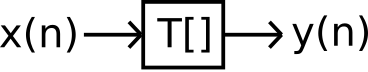
\includegraphics[width=0.3\linewidth]{img/img01}
	\end{figure}
	\begin{itemize}
		\item General: \[ y(n) = T[x(n)] \]
		\item LSI: 
		\begin{align*}
			y(n) &= \sum_{k=-\infty}^{+\infty} x(k)h(n-k) \\
				 &= \sum_{k=-\infty}^{+\infty} h(k)x(n-k)
		\end{align*}
		\item \textbf{CONVOLUTION SUM}
	\end{itemize}
\end{frame}

\begin{frame}
	\frametitle{Stability}
	
	\begin{definition}
		If x(n) bounded, i.e. $ |x(n)| < \infty $ all $ n $ then $ y(n) $ bounded, i.e. $ |y(n)| < \infty $ all $ n $
	\end{definition}

	\begin{itemize}
		\item LSI: \[ \sum_{k = -\infty}^{+\infty} |h(k)|  < \infty \]
		\item Exp:
		\begin{align*}
			h(n) &= 2^n u(n) \leftarrow \text{unstable} \\
			h(n) &= (\frac{1}{2})^n u(n) \leftarrow \text{stable}
		\end{align*}
	\end{itemize}
\end{frame}

\begin{frame}
	\frametitle{Causality}
	
	\begin{definition}
		$ y(n) $ for $ n=n $, depends on $ x(n) $ only for $ n \leq n $
	\end{definition}
	
	\begin{itemize}
		\item LSI: \[ h(n) = 0 ~ n < 0 \]
		\item Exp:
		\begin{align*}
		h(n) &= 2^n u(-n) \leftarrow \text{noncausal \& stable}
		\end{align*}
	\end{itemize}
\end{frame}

\section{Linear Constant Coefficient Difference Equation}

\begin{frame}
	\frametitle{Linear Constant Coefficient Difference Equation}
	\begin{itemize}
		\item $ N^{th} $ order
		\[ \sum_{k = 0}^N a_k y(n-k) = \sum_{r = 0}^M b_r x(n-r) \]
		\item $ N = 0 $, $ a_0 = 1 $
		\begin{align*}
		y(n) &= \sum_{r = 0}^M b_r x(n-r) \\
		h(n) &= b_n;~n = 0, 1, \dots, M \\
		     &= 0;~\text{otherwise}
		\end{align*}
		
	\end{itemize}
\end{frame}

\begin{frame}
	\frametitle{Linear Constant Coefficient Difference Equation}
	\begin{itemize}
		\item $ \text{N}^\text{th} $order
		\[ \sum_{k = 0}^N a_k y(n-k) = \sum_{r = 0}^M b_r x(n-r) \]
		\item $ N \neq 0 $, $ a_0 = 1 $
		\begin{align*}
		y(n) &= \sum_{r = 0}^M b_r x(n-r) - \sum_{k = 1}^N a_k y(n-k) \\
		\end{align*}
	\end{itemize}
\end{frame}

\begin{frame}
	\frametitle{Linear Constant Coefficient Difference Equation}
	\begin{itemize}
		\item First-order
		\[ y(n) - ay(n-1) = x(n) \]
		\[ x(n) = \delta(n) \]
		\item{} assume $ y(n) = 0 $ for $ n<0 $
		\[ y(n) = \delta(n) + ay(n-1) \]
		\[
			\begin{rcases*}
			y(-1)= 0 \\
			y(0) = 1 \\
			y(1) = a \\
			y(2) = a^2
			\end{rcases*} a^n u(n);~|a|<1 \rightarrow \text{stable}
		\]
	\end{itemize}
\end{frame}

\begin{frame}
	\frametitle{Linear Constant Coefficient Difference Equation}
	\begin{itemize}
		\item First-order
		\[ y(n) - ay(n-1) = x(n) \]
		\[ x(n) = \delta(n) \]
		\item{} assume $ y(n) = 0 $ for $ n>0 $
		\[ y(n-1) = a^{-1}[y(n) - \delta(n)] \]
		\[
		\begin{rcases*}
		y(1)= 0 \\
		y(0) = 0 \\
		y(-1) = -a^{-1} \\
		y(-2) = -a^{-2}
		\end{rcases*} -a^n u(-n-1);~|a|<1 \rightarrow \text{unstable}
		\]
	\end{itemize}
\end{frame}

\begin{frame}
	\frametitle{Linear Constant Coefficient Difference Equation}
	\begin{alertblock}{Conclussion}
		\begin{itemize}
			\item Linear constant coefficient difference equation doesn't specify uniquely a sistem, it requires a set of initial conditions.
			\item Depending on the initial conditions or boundary conditions that are imposed, it may correspond to a causal system, or it may correspond to a non-causal system.
		\end{itemize}
	\end{alertblock}
\end{frame}

\section{Frequency Response of LSI Systems}

\begin{frame}
	\frametitle{Frequency Response of LSI Systems}
	\begin{itemize}
		\item Frequency Response
		\[ y(n) = \sum_{k = -\infty}^{+\infty} h(k) x(n-k)\]
		\item[] Let $ x(n) = e^{j\omega n} $
		\begin{align*}
			y(n) &= \sum_{k = -\infty}^{+\infty} h(k) e^{j\omega (n - k)} \\
			&= (e^{j\omega n} ) \sum_{k = -\infty}^{+\infty} h(k) e^{-j\omega k} \\ 
			&= H(e^{j\omega}) e^{j\omega n} \\
			H(e^{j\omega}) &=  \sum_{n = -\infty}^{+\infty} h(n) e^{-j\omega n}
		\end{align*}
	\end{itemize}
\end{frame}

\begin{frame}
	\frametitle{Frequency Response of LSI Systems}
	\begin{itemize}
		\item Sinusoidal Response
		\begin{align*}
			x(n) &= A\cos (\omega_0 n + \phi) \\ 
			&= \frac{A}{2}e^{j \phi} e^{j\omega_0n} + \frac{A}{2}e^{-j \phi} e^{-j\omega_0n}
		\end{align*}
		\item Freq. Response in polar form
		\[ H(e^{j\omega_0}) = |H(e^{j\omega_0})| e^{j\theta(\omega_0)} \]
		\item Result
		\[ y(n) = |H(e^{j\omega_0})| . \cos (\omega_0 n + \phi + \theta)  \]
	\end{itemize}
\end{frame}

\begin{frame}
	\frametitle{Frequency Response of LSI Systems}
	\begin{itemize}
		\item Example:
		\[ y(n) - ay(n-1) = x(n)  \]
		\item Causal
		\[ h(n) = a^n u(n)~~0<a<1 \]
		\begin{align*}
			H(e^{j\omega}) &= \sum_{n = -\infty}^{+\infty}a^n u(n) e^{-j\omega n} \\
			&= \sum_{n = 0}^{\infty} {(ae^{-j\omega})}^n  = \sum_{n = 0}^{\infty} \alpha^n \\
			&= \frac{1}{1 - ae^{-j\omega}}
		\end{align*}
	\end{itemize}
\end{frame}

\begin{frame}
	\frametitle{Frequency Response of LSI Systems}
	\begin{itemize}
		\item Magnitude of frequency response
			\begin{align*}
				{|H(e^{j\omega})|}^2 &= \frac{1}{1 - ae^{j\omega}} . \frac{1}{1 - ae^{-j\omega}} \\
				&= \frac{1}{1 + a^2 - 2a\cos \omega}
			\end{align*}
		\item Phase angle
		\[ \measuredangle H(e^{j\omega}) = \tan^{-1}\left[ \frac{-a\sin \omega}{1 - a\cos \omega} \right] \]
	\end{itemize}
\end{frame}

\begin{frame}
	\frametitle{Frequency Response of LSI Systems}
	\begin{center}
		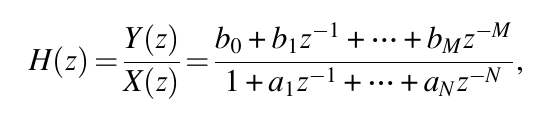
\includegraphics[width=0.7\linewidth]{img/img02}
	\end{center}
\end{frame}

\begin{frame}
	\frametitle{Properties of Frequency Response}
	\begin{enumerate}
		\item Function of continuous variable $ \omega $
		\item Periodic function of $ \omega $  period 2$\pi$
	\end{enumerate}
	\begin{equation*}
		e^{j(\omega + 2 \pi k)n} = e^{j \omega n} e^{j 2 \pi k n}
	\end{equation*}
	\begin{itemize}
		\item Generalization The Fourier Transform
	\end{itemize}
\end{frame}

\end{document}